\begin{frame}{Stav práce}{Výsledky měření - Zápis}
\begin{center}
   \vspace{-0.2cm}
   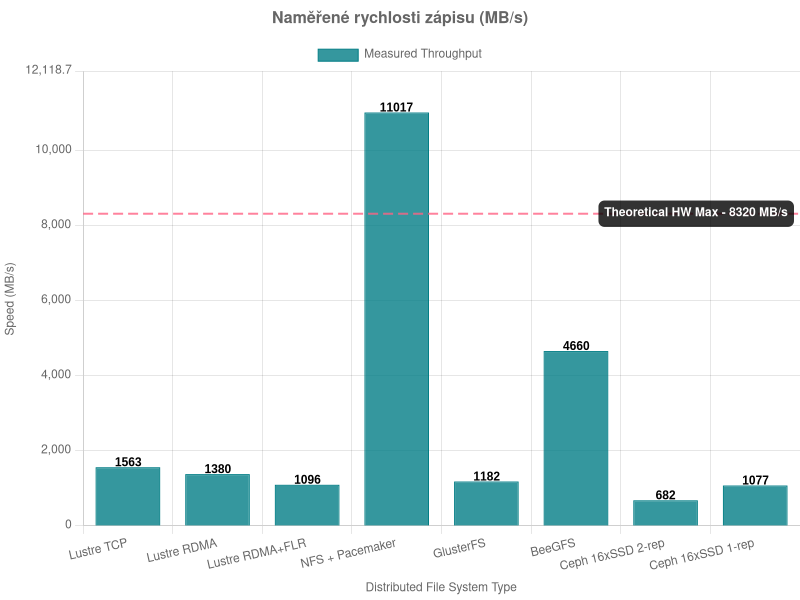
\includegraphics[width=0.65\textwidth]{assets/write_performance.png}
\end{center}
\note{
\begin{itemize}
 \item \textbf{NFS + Pacemaker} je outlier .... cache v paměti a když to bylo zakázáno v CFG
 \item \textbf{NFS + Pacemaker} NUKE + velice riskatní protože hlava dělá veškerou logiku RAID arr
 \item \textbf{BeegFS} Super výsledke ... ALE v CE je jen RAID 0 ... nelze použit v PROD
\end{itemize}
}
\end{frame}

